
% {
% \setbeamertemplate{footline}{}
% \begin{frame}
% \begin{block}{}
% \begin{quote}
% The only thing that is constant is change.\\
% \hfill Heraclitus of Ephesus
% \end{quote}
% \end{block}
% \end{frame}
% }

% {
% \setbeamertemplate{footline}{}
% \begin{frame}{}%{A Sub-title is optional}
% \begin{center}
\includegraphics[clip=true, scale=0.91, trim=100 0 100 0]{images/3rdparty/obama-change}\end{center}
% \end{frame}
% }

\section{Introduction}
% \subsection{Motivation}
\begin{frame}{Motivation}%{A Sub-title is optional}
\begin{itemize}
\item Software applications change all the time
\item Deployed systems must be updated with bug fixes, new features
\item Updating typically involves: stop, apply patch, restart
% \vspace{1ex}
% \begin{center}\begin{Huge}Updating $\Rightarrow$ Downtime\end{Huge}\end{center}
% \item Not desirable
%   \begin{itemize}
%     \item Safety concerns
%     \item Revenue loss
%     \item Inconvenience
%   \end{itemize}
\end{itemize}
% \item Might not be affordable for some applications
%   \begin{itemize}
%   \item Applications that retain state that cannot be externalized
%   \end{itemize}
\end{frame}

\begin{frame}{}%{A Sub-title is optional}
\only<3->{\begin{textblock*}{0mm}[0,0](40mm,25mm)
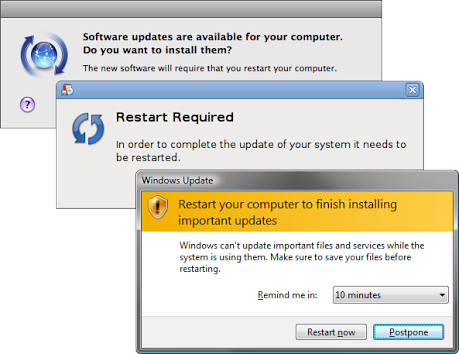
\includegraphics[scale=0.6,clip=true]{images/3rdparty/restart-required}%
\end{textblock*}}
\only<2->{\begin{textblock*}{0mm}[0,0](10mm,55mm)
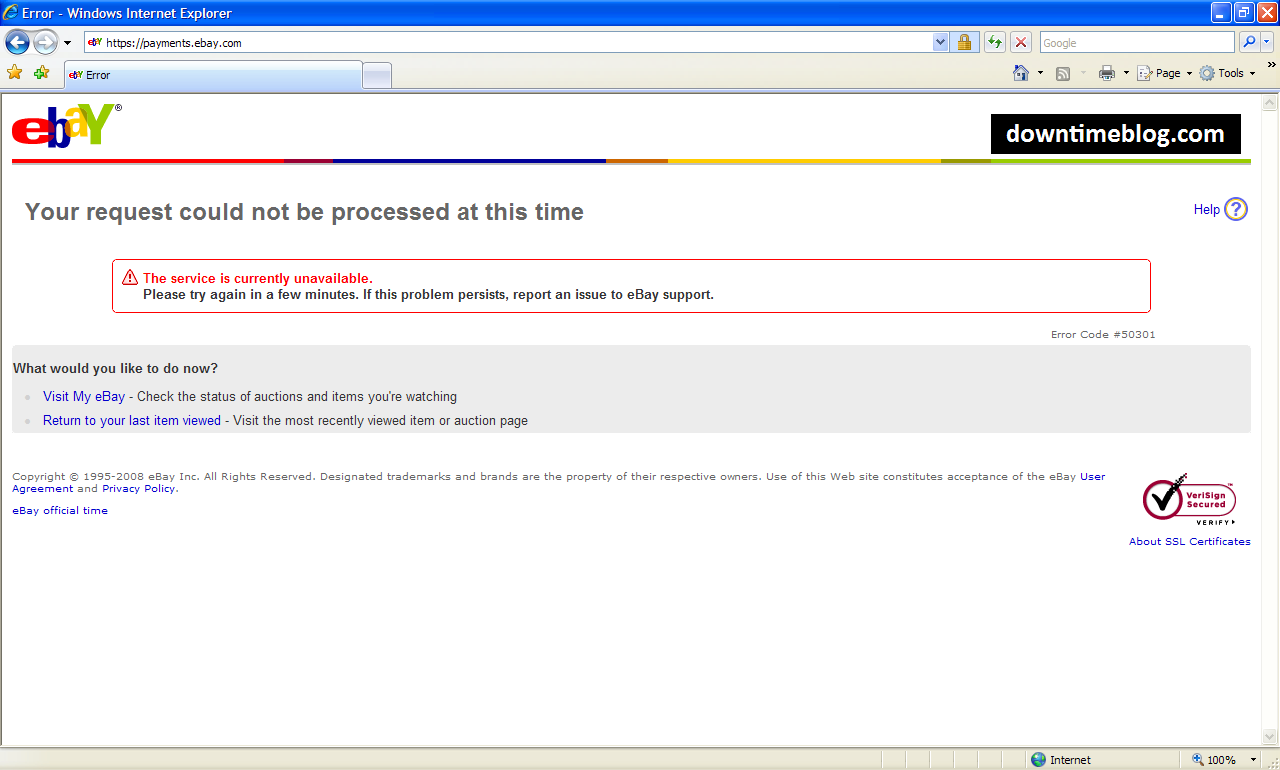
\includegraphics[scale=0.4,clip=true,trim=0 450 525 90]{images/3rdparty/ebay-downtime}%
\end{textblock*}}
\begin{textblock*}{0mm}[0,0](5mm,5mm)
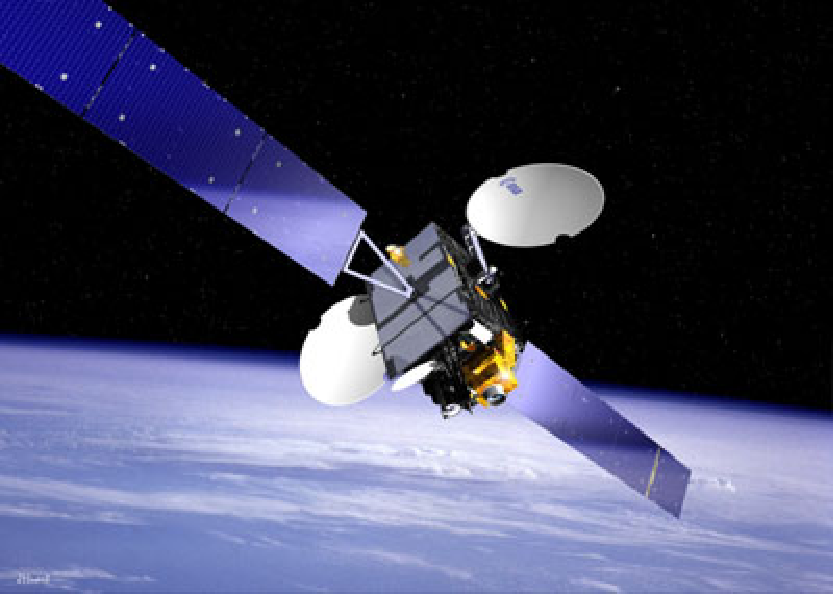
\includegraphics[scale=0.5,clip=true,angle=15,trim=0 30 35 0]{images/3rdparty/esa-satellite}%
\end{textblock*}
\end{frame}

\begin{frame}{}%{A Sub-title is optional}
\begin{block}{}
\begin{center}
{\LARGE
The fundamental problem is losing state because of downtime.
}
\vspace{0.5ex}
\end{center}
\end{block}
\end{frame}

\begin{frame}{Dynamic software updating}%{A Sub-title is optional}
\vspace*{-3mm}%
\begin{center}%
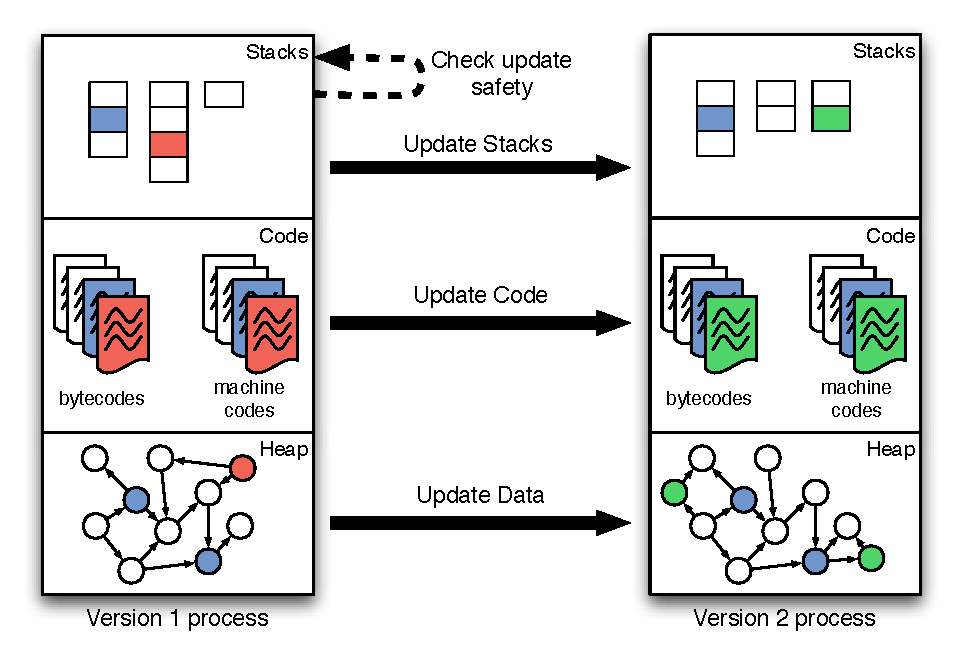
\includegraphics[scale=0.73]{images/process-state/both-process-state}%
\end{center}%
\end{frame}

\begin{frame}{Overheard on programming.reddit}%{A Sub-title is optional}
\only<1->{\begin{textblock*}{0mm}[0,0](24mm,38mm)
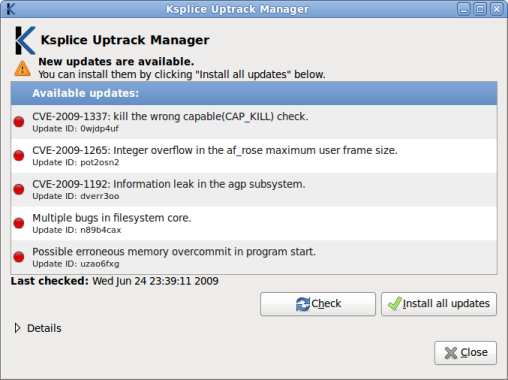
\includegraphics[,clip=true,scale=0.3,angle=345]{images/3rdparty/ksplice}%
\end{textblock*}}
\only<1->{\begin{textblock*}{0mm}[0,0](64mm,6mm)

\includegraphics[,clip=true,scale=1.00,angle=330]{images/3rdparty/erlang}%
\end{textblock*}}
\only<1->{\begin{textblock*}{0mm}[0,0](00mm,00mm)

\includegraphics[,clip=true,scale=0.35,angle=30,trim=0 0 420 0]{images/3rdparty/jetpack}%
\end{textblock*}}
\end{frame}

\begin{frame}{Dynamic updating systems}%{A Sub-title is optional}
\begin{itemize}
\item Special-purpose architectures, application-specific solutions exist
\item General-purpose solutions gaining strength
  \begin{itemize}
  \item K42, Ksplice for OS updates
  \item Polus, Ginseng for C applications
  \end{itemize}
\item Not for managed languages
\end{itemize}
\end{frame}

% \begin{frame}{DSU opportunity for managed languages}%{A Sub-title is optional}
% DSU Solutions for C/C++ typically
% \begin{itemize}
% \item Require special compilation
% \item Statically/dynamically insert indirection for function calls
% \item Restrict structure updates, require extra allocation
% \item Impose space/time overheads on normal execution
% \item Make type-safety for updates difficult
% \item Not multi-threaded
% \end{itemize}
% \end{frame}

% \begin{frame}{DSU requirements}%{A Sub-title is optional}
% % \begin{center}
% % A Dynamic Software Updating solution should \emph{ideally} be
% % {\bf safe}, {\bf flexible}, and {\bf efficient}.
% % \end{center}
% \begin{description}
% \item[Safe] Updating is as correct as starting from scratch
% \item[Flexible] Support changes encountered in practice
% \item[Efficient] No performance impact
% \end{description}
% \end{frame}

% \begin{frame}{State of the art}%{A Sub-title is optional}
% Significant progress for C
% \begin{itemize}
% \item Server feature upgrades
%   \begin{itemize}
%   \item Ginseng \cite{neamtiu06dsu}
%   \item POLUS \cite{chen:icse07}
%   \end{itemize}
% \item Security patches: OPUS \cite{altekar05opus}
% \item Operating system upgrades
%   \begin{itemize}
%   \item K42 \cite{K42reconfig}
%   \item DynAMOS \cite{dynamos_eurosys_07}
%   \item LUCOS \cite{chen06vee}
%   \item Ksplice \cite{Ksplice}
%   \end{itemize}
% \end{itemize}
% % \item<2-> Primitive support for managed languages
% %   \begin{itemize}
% %   \item Very restrictive
% %   \item Space and time overheads
% %   \item Not proven on realistic applications
% %   \end{itemize}
% \end{frame}

% \begin{frame}{Possible DSU solutions}%{A Sub-title is optional}
% Achieve DSU support by
% \begin{itemize}
% \item Making the application DSU-aware
% \item Special recompilation
% \item A class loader based colution 
% \item DSU support in the VM
% \end{itemize}
% \end{frame}

% \begin{frame}{Related work}%{A Sub-title is optional}
% \begin{itemize}
% \item Custom class loader solutions:\\Eisenbach and Barr, Milazzo et al.
% \item Source-to-source translation: Orso et al.
% \item VM-based solutions: JDrums, Dynamic Virtual Machine (DVM)
% \item In a persistent object store: Boyapati et al.
% \end{itemize}
% \uncover<2>{
% \begin{itemize}
% \item Limited, not flexible
% \item Restricted data-transformation model (like requiring {\em encapsulation} based
% on {\em ownership types})
% \item Overhead during normal execution
% \end{itemize}
% }
% \end{frame}

% \begin{frame}{Existing solutions for managed languages}%{A Sub-title is optional}
% \begin{itemize}
% \item VM-based solutions
%   \begin{itemize}
%   \item JDrums \cite{ritzau00dynamic}, DVM \cite{Mala00a}
%   \item Not well evaluated
%   \item Provide an interface similar to \DSU{}
%   \item Perform lazy updates
%   \item Overheads during normal execution
%   \end{itemize}
% \item Standard VM with DSU support
%   \begin{itemize}
%   \item DJVCS \cite{BarrE03}, DUSC \cite{orso:java}, \cite{Milazzo05updates}
%   \item Special classloaders, compilers
%   \item Very restrictive
%   \item Space/time overheads
%   \end{itemize}
% \end{itemize}
% 
% \end{frame}

% \begin{frame}{Related work}%{A Sub-title is optional}
% Nobody can beat us.
% \end{frame}

\begin{frame}{Our solution}%{A Sub-title is optional}
\begin{itemize}
\item \DSU{} - a Java Virtual Machine with DSU support
% \item Built on top of Jikes RVM, a Java-in-Java VM
\item Key insight: Extend existing VM services
%   \begin{itemize}
%   \item Classloading
%   \item Bytecode verification%\footnote{Jikes RVM does not have a bytecode verifier}
%   \item Thread synchronization
%   \item JIT Compilation
%   \item On-stack replacement
%   \item Garbage collection
%   \end{itemize}
\item No DSU-related overhead during normal execution
\item Support updates to real world applications
\begin{block}{}
\emph{Dynamic software updating in managed languages can be achieved in a
{\bf safe}, {\bf flexible} and {\bf efficient} manner by naturally extending existing VM
services.}
\end{block}

\begin{block}{}
\emph{DSU support should be a standard feature of future VMs.}
\end{block}
\end{itemize}
\end{frame}
